% Revised Scenario-B protocol (honest-but-curious). Build: pdflatex protocol_v2.tex
\documentclass[tikz,border=8pt]{standalone}
\usepackage{amsmath,amssymb,array}
\usepackage[T1]{fontenc}
\IfFileExists{lmodern.sty}{\usepackage{lmodern}}{}
\usetikzlibrary{arrows.meta,positioning,calc,backgrounds,fit}

\definecolor{newc}{RGB}{196,90,12}     % new / changed vs the draft protocol
\definecolor{oldc}{RGB}{110,110,110}   % unchanged
\definecolor{rlane}{RGB}{232,240,250}
\definecolor{olane}{RGB}{236,246,236}

\tikzset{
  box/.style={rectangle, rounded corners=2pt, draw=oldc, fill=white, line width=0.5pt,
              text width=7.0cm, align=left, font=\footnotesize, inner sep=4pt},
  newbox/.style={box, draw=newc, fill=newc!6, line width=0.9pt},
  msg/.style={-{Stealth[length=2.6mm]}, line width=0.7pt, draw=oldc},
  newmsg/.style={msg, draw=newc, line width=1pt},
  mlabel/.style={font=\scriptsize, text width=3.9cm, align=center, inner sep=1.5pt},
  phase/.style={rectangle, fill=black!78, text=white, font=\small\bfseries,
                minimum width=19.6cm, minimum height=5.2mm, anchor=north west, inner xsep=6pt,
                text width=19cm, align=left},
  badge/.style={circle, fill=newc, text=white, font=\scriptsize\bfseries, inner sep=0pt,
                minimum size=4.2mm},
  head/.style={rectangle, rounded corners=3pt, text width=7.0cm, align=center,
               font=\small, inner sep=5pt, draw=black!60},
}
% badges sit outside the boxes: right of O's boxes, left of R's boxes; third arg = stack index
\newcommand{\obdg}[3]{\node[badge] at ($(#1.north east)+(0.34,{-0.28-0.5*#3})$) {#2};}
\newcommand{\rbdg}[3]{\node[badge] at ($(#1.north west)+(-0.34,{-0.28-0.5*#3})$) {#2};}

\begin{document}
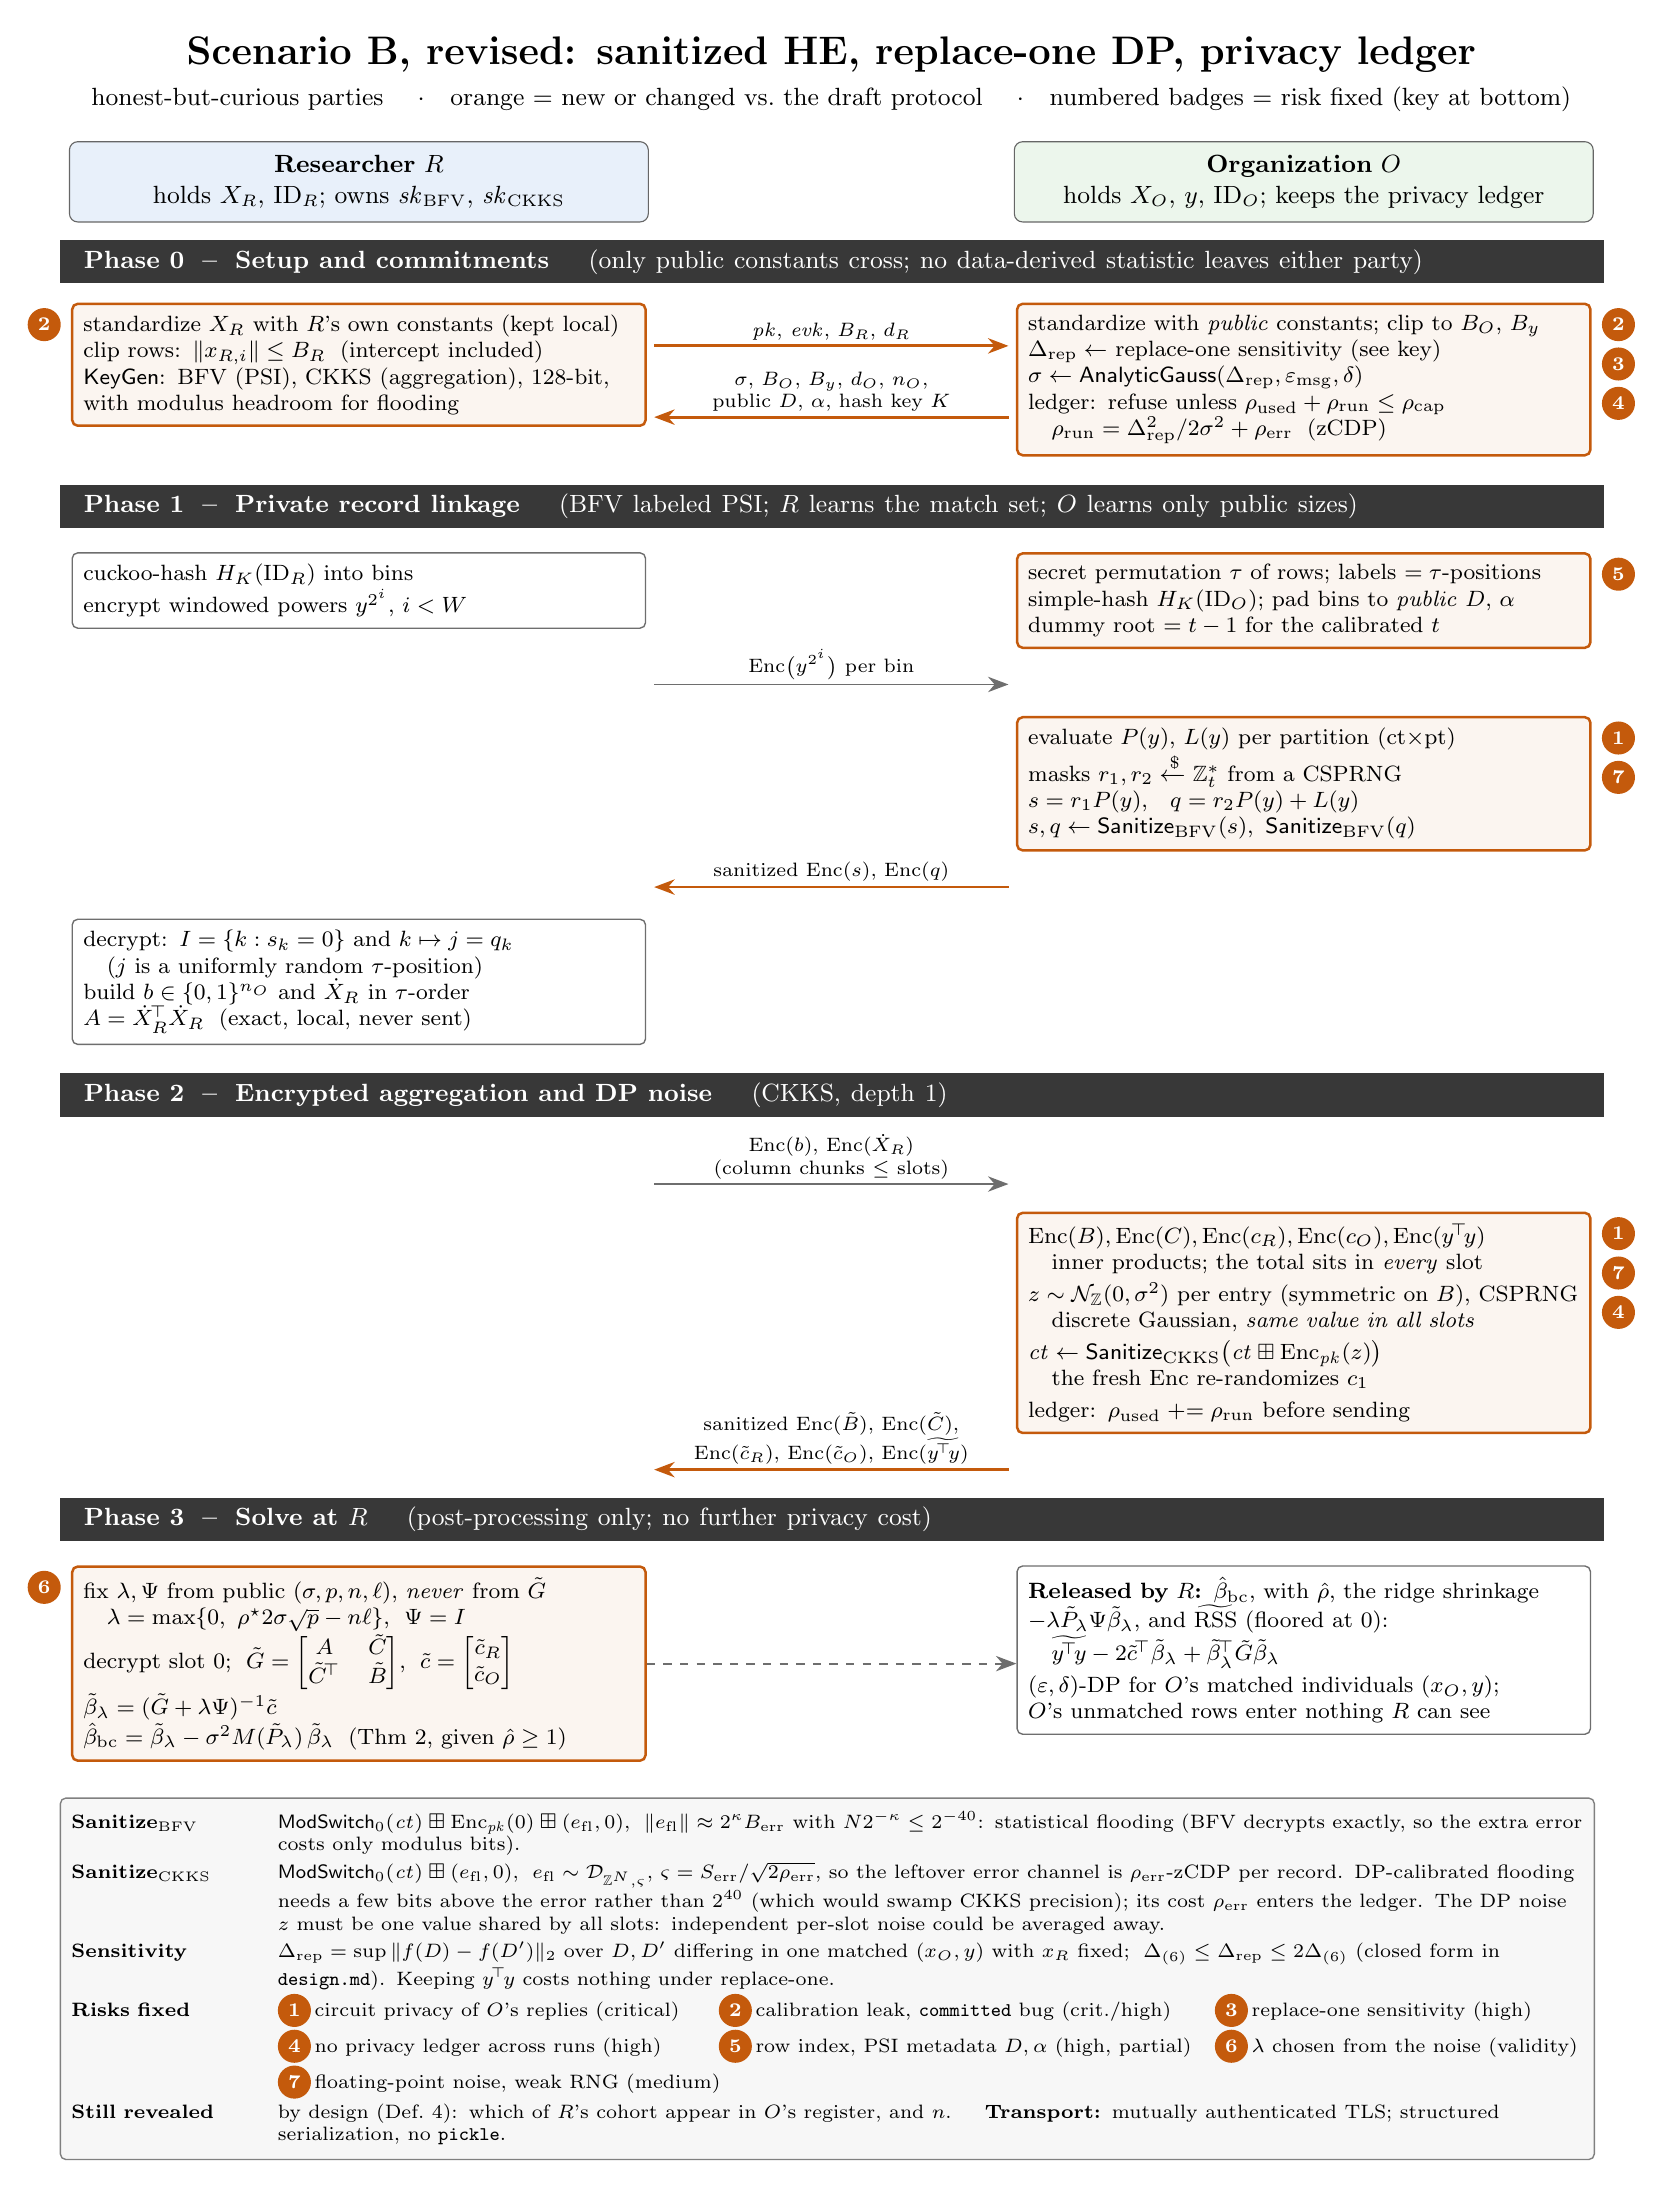
\begin{tikzpicture}
% x layout: R lane centred at 0 (box -3.7..3.7), O lane centred at 12 (8.3..15.7)
\def\RL{3.75}\def\OL{8.25}

\node[font=\Large\bfseries, anchor=south] at (6,1.45) {Scenario B, revised: sanitized HE, replace-one DP, privacy ledger};
\node[font=\small, anchor=south] at (6,0.95) {honest-but-curious parties \quad$\cdot$\quad orange $=$ new or changed vs.\ the draft protocol \quad$\cdot$\quad numbered badges $=$ risk fixed (key at bottom)};

\node[head, fill=rlane, anchor=north] (hR) at (0,0.7) {\textbf{Researcher $R$}\\ holds $X_R$, $\mathrm{ID}_R$; owns $\mathit{sk}_{\mathrm{BFV}}$, $\mathit{sk}_{\mathrm{CKKS}}$};
\node[head, fill=olane, anchor=north] (hO) at (12,0.7) {\textbf{Organization $O$}\\ holds $X_O$, $y$, $\mathrm{ID}_O$; keeps the privacy ledger};

% ---------------- Phase 0 ----------------
\node[phase] (p0) at (-3.8,-0.55) {Phase 0 \;--\; Setup and commitments \quad {\normalfont (only public constants cross; no data-derived statistic leaves either party)}};
\node[newbox, anchor=north] (r0) at (0,-1.35) {%
  standardize $X_R$ with $R$'s own constants (kept local)\\
  clip rows: $\|x_{R,i}\|\le B_R$ \;(intercept included)\\
  \textsf{KeyGen}: BFV (PSI), CKKS (aggregation), 128-bit,\\
  with modulus headroom for flooding};
\node[newbox, anchor=north] (o0) at (12,-1.35) {%
  standardize with \emph{public} constants; clip to $B_O$, $B_y$\\
  $\Delta_{\mathrm{rep}}\leftarrow$ replace-one sensitivity (see key)\\
  $\sigma\leftarrow\textsf{AnalyticGauss}(\Delta_{\mathrm{rep}},\varepsilon_{\mathrm{msg}},\delta)$\\
  ledger: refuse unless $\rho_{\mathrm{used}}+\rho_{\mathrm{run}}\le\rho_{\mathrm{cap}}$\\
  \hspace*{1em}$\rho_{\mathrm{run}}=\Delta_{\mathrm{rep}}^2/2\sigma^2+\rho_{\mathrm{err}}$ \;(zCDP)};
\rbdg{r0}{2}{0}
\obdg{o0}{2}{0}\obdg{o0}{3}{1}\obdg{o0}{4}{2}
\coordinate (a0) at ($(r0.north)+(0,-0.55)$);
\draw[newmsg] (\RL,0 |- a0) -- node[mlabel, above] {$\mathit{pk}$, $\mathit{evk}$, $B_R$, $d_R$} (\OL,0 |- a0);
\coordinate (a0b) at ($(o0.south)+(0,0.5)$);
\draw[newmsg] (\OL,0 |- a0b) -- node[mlabel, above] {$\sigma$, $B_O$, $B_y$, $d_O$, $n_O$,\\ public $D$, $\alpha$, hash key $K$} (\RL,0 |- a0b);

% ---------------- Phase 1 ----------------
\node[phase] (p1) at ($(-3.8,0 |- o0.south)+(0,-0.35)$) {Phase 1 \;--\; Private record linkage \quad {\normalfont (BFV labeled PSI; $R$ learns the match set; $O$ learns only public sizes)}};
\node[box, anchor=north] (r1) at ($(0,0 |- p1.south)+(0,-0.3)$) {%
  cuckoo-hash $H_K(\mathrm{ID}_R)$ into bins\\
  encrypt windowed powers $y^{2^i}$, $i<W$};
\node[newbox, anchor=north] (o1) at ($(12,0 |- p1.south)+(0,-0.3)$) {%
  secret permutation $\tau$ of rows; labels $=\tau$-positions\\
  simple-hash $H_K(\mathrm{ID}_O)$; pad bins to \emph{public} $D$, $\alpha$\\
  dummy root $=t-1$ for the calibrated $t$};
\obdg{o1}{5}{0}
\coordinate (a1) at ($(o1.south)+(0,-0.45)$);
\draw[msg] (\RL,0 |- a1) -- node[mlabel, above] {$\mathrm{Enc}\big(y^{2^i}\big)$ per bin} (\OL,0 |- a1);
\node[newbox, anchor=north] (o1b) at ($(12,0 |- a1)+(0,-0.4)$) {%
  evaluate $P(y)$, $L(y)$ per partition (ct$\times$pt)\\
  masks $r_1,r_2\xleftarrow{\$}\mathbb{Z}_t^{\ast}$ from a CSPRNG\\
  $s=r_1P(y)$, \; $q=r_2P(y)+L(y)$\\
  $s,q\leftarrow\textsf{Sanitize}_{\mathrm{BFV}}(s),\ \textsf{Sanitize}_{\mathrm{BFV}}(q)$};
\obdg{o1b}{1}{0}\obdg{o1b}{7}{1}
\coordinate (a1b) at ($(o1b.south)+(0,-0.45)$);
\draw[newmsg] (\OL,0 |- a1b) -- node[mlabel, above] {sanitized $\mathrm{Enc}(s)$, $\mathrm{Enc}(q)$} (\RL,0 |- a1b);
\node[box, anchor=north] (r1b) at ($(0,0 |- a1b)+(0,-0.4)$) {%
  decrypt: $I=\{k: s_k=0\}$ and $k\mapsto j=q_k$\\
  \hspace*{1em}($j$ is a uniformly random $\tau$-position)\\
  build $b\in\{0,1\}^{n_O}$ and $\dot X_R$ in $\tau$-order\\
  $A=\dot X_R^{\!\top}\dot X_R$ \;(exact, local, never sent)};

% ---------------- Phase 2 ----------------
\node[phase] (p2) at ($(-3.8,0 |- r1b.south)+(0,-0.35)$) {Phase 2 \;--\; Encrypted aggregation and DP noise \quad {\normalfont (CKKS, depth 1)}};
\coordinate (a2) at ($(p2.south)+(0,-0.85)$);
\draw[msg] (\RL,0 |- a2) -- node[mlabel, above] {$\mathrm{Enc}(b)$, $\mathrm{Enc}(\dot X_R)$\\ (column chunks $\le$ slots)} (\OL,0 |- a2);
\node[newbox, anchor=north] (o2) at ($(12,0 |- a2)+(0,-0.35)$) {%
  $\mathrm{Enc}(B),\mathrm{Enc}(C),\mathrm{Enc}(c_R),\mathrm{Enc}(c_O),\mathrm{Enc}(y^{\!\top}\!y)$\\
  \hspace*{1em}inner products; the total sits in \emph{every} slot\\[2pt]
  $z\sim\mathcal{N}_{\mathbb{Z}}(0,\sigma^2)$ per entry (symmetric on $B$), CSPRNG\\
  \hspace*{1em}discrete Gaussian, \emph{same value in all slots}\\[2pt]
  $\mathit{ct}\leftarrow\textsf{Sanitize}_{\mathrm{CKKS}}\big(\mathit{ct}\boxplus\mathrm{Enc}_{\mathit{pk}}(z)\big)$\\
  \hspace*{1em}the fresh $\mathrm{Enc}$ re-randomizes $c_1$\\[2pt]
  ledger: $\rho_{\mathrm{used}}\mathrel{+}=\rho_{\mathrm{run}}$ before sending};
\obdg{o2}{1}{0}\obdg{o2}{7}{1}\obdg{o2}{4}{2}
\coordinate (a2b) at ($(o2.south)+(0,-0.45)$);
\draw[newmsg] (\OL,0 |- a2b) -- node[mlabel, above] {sanitized $\mathrm{Enc}(\tilde B)$, $\mathrm{Enc}(\tilde C)$,\\ $\mathrm{Enc}(\tilde c_R)$, $\mathrm{Enc}(\tilde c_O)$, $\mathrm{Enc}(\widetilde{y^{\!\top}\!y})$} (\RL,0 |- a2b);

% ---------------- Phase 3 ----------------
\node[phase] (p3) at ($(-3.8,0 |- a2b)+(0,-0.35)$) {Phase 3 \;--\; Solve at $R$ \quad {\normalfont (post-processing only; no further privacy cost)}};
\node[newbox, anchor=north] (r3) at ($(0,0 |- p3.south)+(0,-0.3)$) {%
  fix $\lambda,\Psi$ from public $(\sigma,p,n,\ell)$, \emph{never} from $\tilde G$\\
  \hspace*{1em}$\lambda=\max\{0,\ \rho^\star 2\sigma\sqrt p-n\ell\}$, \;$\Psi=I$\\
  decrypt slot 0; \;$\tilde G=\begin{bmatrix}A&\tilde C\\ \tilde C^{\!\top}&\tilde B\end{bmatrix}$, \;$\tilde c=\begin{bmatrix}\tilde c_R\\ \tilde c_O\end{bmatrix}$\\
  $\tilde\beta_\lambda=(\tilde G+\lambda\Psi)^{-1}\tilde c$\\
  $\hat\beta_{\mathrm{bc}}=\tilde\beta_\lambda-\sigma^2M(\tilde P_\lambda)\,\tilde\beta_\lambda$ \;(Thm 2, given $\hat\rho\ge1$)};
\rbdg{r3}{6}{0}
\node[box, anchor=north, text width=7.0cm] (out) at ($(12,0 |- p3.south)+(0,-0.3)$) {%
  \textbf{Released by $R$:} $\hat\beta_{\mathrm{bc}}$, with $\hat\rho$, the ridge shrinkage\\
  $-\lambda\tilde P_\lambda\Psi\tilde\beta_\lambda$, and $\widetilde{\mathrm{RSS}}$ (floored at 0):\\
  \hspace*{1em}$\widetilde{y^{\!\top}\!y}-2\tilde c^{\!\top}\tilde\beta_\lambda+\tilde\beta_\lambda^{\!\top}\tilde G\tilde\beta_\lambda$\\[2pt]
  $(\varepsilon,\delta)$-DP for $O$'s matched individuals $(x_O,y)$;\\
  $O$'s unmatched rows enter nothing $R$ can see};
\draw[msg, dashed] (r3.east) -- (out.west |- r3.east);

% ---------------- Key ----------------
\newcommand{\B}[1]{\tikz[baseline=(b.base)]\node[badge](b){#1};}
\node[box, anchor=north west, text width=19.2cm, draw=black!50, fill=black!3, font=\scriptsize] (key) at ($(-3.8,0 |- r3.south)+(0,-0.45)$) {%
  \renewcommand{\arraystretch}{1.25}%
  \begin{tabular}{@{}p{2.2cm}>{\raggedright\arraybackslash}p{16.6cm}@{}}
  \textbf{Sanitize$_{\mathrm{BFV}}$} & $\textsf{ModSwitch}_0(\mathit{ct})\boxplus\mathrm{Enc}_{\mathit{pk}}(0)\boxplus(e_{\mathrm{fl}},0)$, \;$\|e_{\mathrm{fl}}\|\approx2^{\kappa}B_{\mathrm{err}}$ with $N2^{-\kappa}\le2^{-40}$: statistical flooding (BFV decrypts exactly, so the extra error costs only modulus bits).\\
  \textbf{Sanitize$_{\mathrm{CKKS}}$} & $\textsf{ModSwitch}_0(\mathit{ct})\boxplus(e_{\mathrm{fl}},0)$, \;$e_{\mathrm{fl}}\sim\mathcal{D}_{\mathbb{Z}^N,\varsigma}$, $\varsigma=S_{\mathrm{err}}/\sqrt{2\rho_{\mathrm{err}}}$, so the leftover error channel is $\rho_{\mathrm{err}}$-zCDP per record. DP-calibrated flooding needs a few bits above the error rather than $2^{40}$ (which would swamp CKKS precision); its cost $\rho_{\mathrm{err}}$ enters the ledger. The DP noise $z$ must be one value shared by all slots: independent per-slot noise could be averaged away.\\
  \textbf{Sensitivity} & $\Delta_{\mathrm{rep}}=\sup\|f(D)-f(D')\|_2$ over $D,D'$ differing in one matched $(x_O,y)$ with $x_R$ fixed; \;$\Delta_{(6)}\le\Delta_{\mathrm{rep}}\le2\Delta_{(6)}$ (closed form in \texttt{design.md}). Keeping $y^{\!\top}\!y$ costs nothing under replace-one.\\
  \textbf{Risks fixed} &
  \newcommand{\R}[3]{\makebox[#1][l]{\B{#2}\,#3}}%
  \R{5.6cm}{1}{circuit privacy of $O$'s replies (critical)}\R{6.3cm}{2}{calibration leak, \texttt{committed} bug (crit./high)}\R{4.6cm}{3}{replace-one sensitivity (high)}\newline
  \R{5.6cm}{4}{no privacy ledger across runs (high)}\R{6.3cm}{5}{row index, PSI metadata $D,\alpha$ (high, partial)}\R{4.6cm}{6}{$\lambda$ chosen from the noise (validity)}\newline
  \R{5.6cm}{7}{floating-point noise, weak RNG (medium)}\\
  \textbf{Still revealed} & by design (Def.~4): which of $R$'s cohort appear in $O$'s register, and $n$. \quad \textbf{Transport:} mutually authenticated TLS; structured serialization, no \texttt{pickle}.\\
  \end{tabular}};
\end{tikzpicture}
\end{document}
